\section{Experimental Results}\label{sec:experimental-results}

We apply the three different types of models described in Section \ref{sec:classification-methods} to our dataset and evaluate their performance. The natural images are propagated through a CNN pretrained on ImageNet to extract feature vectors. We experiment with both the off-the-shelf features as well as fine-tuning the CNN. When using off-the-shelf features, we simply extract feature vectors and train an SVM on those. For the fine-tuned CNN, we report both results from the softmax classifier used in the actual fine-tuning procedure and training an SVM with extracted fine-tuned feature vectors.  

These extracted feature vectors are also used for VAE and VAE-CCA which makes further compression. We perform classification for those VAE based models by training a classifier, e.g. an SVM, on the data encoded into the latent representation. We use this classification approach for both VAE and VAE-CCA. In all classification experiments, except when we fine-tune the CNN, we use a linear SVM trained with the one-vs-one approach as in \cite{razavian2014cnnfeatures}.

We experiment with three different pretrained CNN architectures, namely AlexNet \cite{krizhevsky2012imagenet}, VGG16 \cite{simonyan2014verydeep} and DenseNet-169 \cite{huang2017densely}. For AlexNet and VGG16, we extract feature vectors of size 4096 from the two last fully connected (FC) layers before the classification layer. The features from the $n^{\text{th}}$ hidden layer are denoted as $\text{AlexNet}_{n}$ and $\text{VGG16}_{n}$. As an example, the last hidden FC layer in AlexNet is denoted as $\text{AlexNet}_{7}$, the input of which is output from $\text{AlexNet}_{6}$. For DenseNet-169, we extract the features of size 1664 from the average pooling layer before its classification layer.

\renewcommand{\arraystretch}{1.2}
\begin{table*}[t]
    \centering
    \caption{ Fine-grained classification (81 classes) accuracies with the methods described in Section \ref{subsec:experimental-setups}. Each row displays from which network architecture and layer that we extracted the feature vectors of the natural images. The columns show the result from the classifiers that we used (see Section \ref{subsec:experimental-setups}). }
    \vspace{2mm}
    \begin{tabular}{c | c c | c c | c c}
        \hline
        \Xhline{3\arrayrulewidth}
        & SVM & SVM-ft & VAE+SVM & VAE+SVM-ft & VAE-CCA+SVM & VAE-CCA+SVM-ft  \\
        \Xhline{3\arrayrulewidth}
        \rowcolor{Gray}
         $\text{AlexNet}_{6}$  &  69.2 & 72.6 & 65.6 & 70.7 & 67.8	& 71.5 \\
         $\text{AlexNet}_{7}$ &  65.0 & 70.7 & 63.0 & 68.7 & 65.0 & 70.9 \\
        \rowcolor{Gray}
         $\text{VGG16}_{6}$ &  62.1	& 73.3 & 57.5 & 71.9 & 60.7 & 73.0 \\
         $\text{VGG16}_{7}$ & 57.3	& 71.7 & 56.8 & 67.8 & 56.8 & 71.3 \\
        \rowcolor{Gray}
         $\text{DenseNet-169}$ & 72.5 & 85.0 & 65.4 & 79.1 & 72.6 & 80.4 \\
        \Xhline{3\arrayrulewidth}
    \end{tabular}
    \label{tab:results-fine-grained}
\end{table*}

\renewcommand{\arraystretch}{1.2}
\begin{table}[t]
    \centering
    \caption{Coarse-grained classification (46 classes) accuracies with an SVM for the methods described in Section \ref{subsec:experimental-setups} that uses off-the-shelf feature representations. Each row displays from network architecture and layer that we extracted the feature vectors of the natural images and the columns show the result for the classification methods. }
    \vspace{2mm}
    \scalebox{0.95}{
    \begin{tabular}{c | ccc}
        \Xhline{3\arrayrulewidth}
         & SVM & VAE+SVM & VAE-CCA+SVM  \\
        \Xhline{3\arrayrulewidth}
        \rowcolor{Gray}
         $\text{AlexNet}_{6}$ & 78.0 & 74.2 & 76.4  \\ 
         $\text{AlexNet}_{7}$ & 75.4 & 73.2 & 74.4  \\ 
        \rowcolor{Gray}
         $\text{VGG16}_{6}$ &  76.6 & 74.2 & 74.9  \\ 
         $\text{VGG16}_{7}$ & 72.8 & 71.7 & 72.3  \\
         \rowcolor{Gray}
         $\text{DenseNet-169}$ & 85.2 & 79.5 & 82.0 \\
        \Xhline{3\arrayrulewidth}
    \end{tabular}
    }
    \label{tab:results-coarse-grained}
\end{table}

\renewcommand{\arraystretch}{1.25}
\begin{table}[t]
\centering
\caption{Fine-grained classification accuracies from fine-tuned CNNs pretrained on ImageNet, where the column shows which architecture that has been fine-tuned. A standard softmax layer is used as the last classification layer.
}
\vspace{2mm}
\scalebox{0.95}{
\begin{tabular}{cccc}
    \hline
    \Xhline{3\arrayrulewidth}
    & AlexNet & VGG16 & DenseNet-169 \\
    \Xhline{3\arrayrulewidth}
    \rowcolor{Gray}
    Fine-tune &  69.3 & 73.8 & 84.0  \\
    \Xhline{3\arrayrulewidth}
\end{tabular}
}
\label{tab:results-finetuned-cnn}
\end{table}


\subsection{Experimental Setups}\label{subsec:experimental-setups}

The following setups were used in the experiments: 


\paragraph*{Setup 1.} Train an SVM on extracted off-the-shelf features from a pretrained CNN, which is denoted as SVM in the results. We also fine-tune the CNN by replacing the final layer with a new softmax layer and denote these results as Fine-tune. We denote training an SVM on extracted finetuned feature vectors as SVM-ft.


\paragraph*{Setup 2.} Extract feature vectors with a pretrained CNN of the natural images and learn a latent representation $\mathbf{z}$ with a VAE. Then the data is encoded into the latent space and we train an SVM with these latent representations, which used for classification. We denote the results as VAE+SVM when using off-the-shelf feature vectors, whereas using the fine-tuned feature vectors are denoted as VAE+SVM-ft. In all experiments with the VAE, we used the architecture from \cite{sohn2015conditionalvae}, i.e. the latent layer having 200 hidden units and both encoder and decoder consisting of two FC layers with 1,000 hidden units each.

\paragraph*{Setup 3.} Each natural image is paired with its corresponding iconic image. We train VAE-CCA similarly as the VAE, but instead, we learn a joint latent representation that is used to reconstruct the extracted feature vectors $\mathbf{x}$ and the iconic images $\mathbf{y}$. The classification is performed with the same steps as in Setup 2 and denotes the results similarly with VAE-CCA+SVM and VAE-CCA+SVM-ft. Our VAE-CCA model takes the feature vectors $\mathbf{x}$ as input and encodes them into a latent layer with 200 hidden units. The encoder and the feature vector decoder uses the same architecture, i.e. two FC layers with 512 hidden units, whereas the iconic image decoder uses the DCGAN \cite{radford2015unsupervised} architecture.

Figure \ref{fig:classification-methods} displays the three experimental setups described above. We report both fine-grained and coarse-grained classification results with an SVM in Table \ref{tab:results-fine-grained} and \ref{tab:results-coarse-grained} respectively. In Table \ref{tab:results-finetuned-cnn}, we report the fine-grained classification results from fine-tuned CNNs.

When fine-tuning the CNNs,
we replace the final layer with a softmax layer applicable to our dataset with randomly initialized weights drawn from a Gaussian with zero mean and standard deviation $0.01$~\cite{Zhang2014PartbasedRCNN}. 
For AlexNet and VGG16, we fine-tune the networks for 30 epochs with two different learning rates, 0.01 for the new classification layer and 0.001 for the pretrained layers. Both learning rates are reduced by half after every fifth epoch. The DenseNet-169 is fine-tuned for 30 epochs with momentum of $0.9$ and an initial learning rate of 0.001, which decays with $10^{-6}$ after each epoch. We report the classification results from the softmax activation after the fine-tuned classification layer. 
We also report classification results from an SVM trained with feature representations from a fine-tuned CNN, which are extracted from FC6 and FC7 of the AlexNet and VGG16 and from the last average pooling layer in DenseNet-169.

The VAE and VAE-CCA models are trained for 50 epochs with Adam \cite{kingma2015adam} for optimizing the ELBOs in Equation \ref{eq:vae-loss} and \ref{eq:vcca-loss} respectively. We use a constant learning rate of 0.0001 and set the minibatch size to 64. The extracted feature vectors are rescaled with standardization before training the VAE and VAE-CCA models to stabilize the learning.

\subsection{Results}
\begin{figure*}[t]
\centering
\subfigure[Royal Gala]{\label{subfig:royal-gala-natural}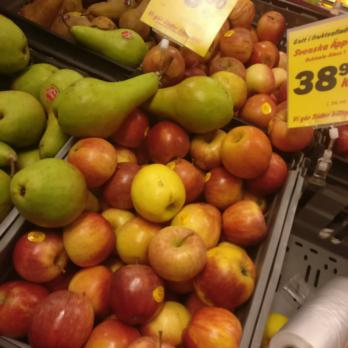
\includegraphics[width=0.33\columnwidth]{decoded-image-figure/Royal-Gala-Apple_003.jpg}}~
\subfigure[Decoded Royal Gala]{\label{subfig:royal-gala-decoded}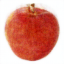
\includegraphics[width=0.33\columnwidth]{decoded-image-figure/densenet_nov11/Royal-Gala-Apple_decoded.png}}~
\subfigure[Brown Cap]{\label{subfig:brown-cap-natural}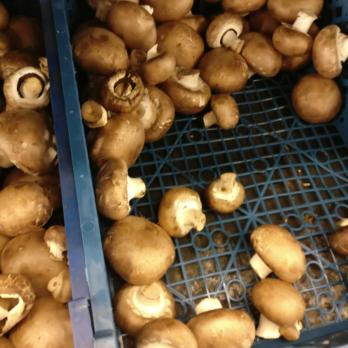
\includegraphics[width=0.33\columnwidth]{decoded-image-figure/Mushroom-Brown-Cap_027.jpg}}~
\subfigure[Decoded\,Brown\,Cap]{\label{subfig:brown-cap-decoded}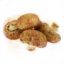
\includegraphics[width=0.33\columnwidth]{decoded-image-figure/densenet_nov11/Mushroom-Brown-Cap_decoded.png}}~
\subfigure[Oatgurt]{\label{subfig:oatgurt-natural}
\includegraphics[width=0.33\columnwidth]{decoded-image-figure/Oatly-Natural-Yoghurt_007.jpg}}~
\subfigure[Decoded Oatgurt]{\label{subfig:oatgurt-decoded}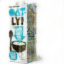
\includegraphics[width=0.33\columnwidth]{decoded-image-figure/densenet_nov11/Oatly-Natural-Yoghurt_decoded.png}}~ \\
\subfigure[Orange]{\label{subfig:orange-natural}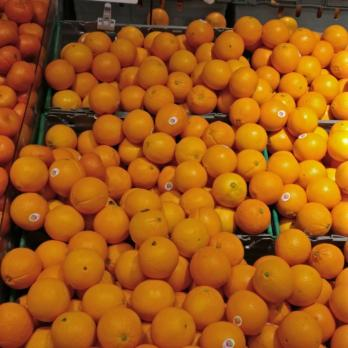
\includegraphics[width=0.33\columnwidth]{decoded-image-figure/Orange_056.jpg}}~
\subfigure[Decoded Orange]{\label{subfig:orange-decoded}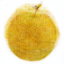
\includegraphics[width=0.33\columnwidth]{decoded-image-figure/densenet_nov11/Orange_decoded.png}}~
\subfigure[Onion]{\label{subfig:onion-natural}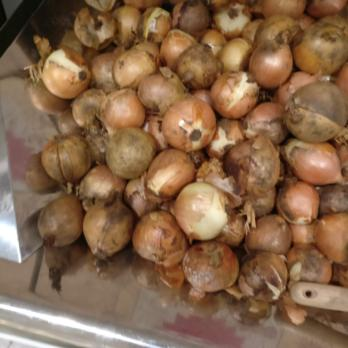
\includegraphics[width=0.33\columnwidth]{decoded-image-figure/Yellow-Onion_030.jpg}}~
\subfigure[Decoded Onion]{\label{subfig:onion-decoded}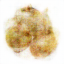
\includegraphics[width=0.33\columnwidth]{decoded-image-figure/densenet_nov11/Yellow-Onion_decoded.png}}~
\subfigure[Yogurt]{\label{subfig:yogurt-natural}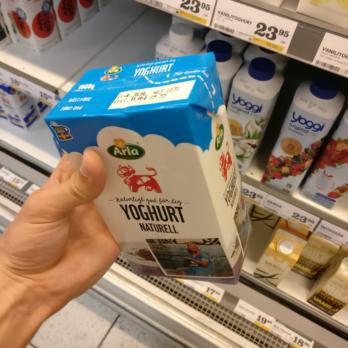
\includegraphics[width=0.33\columnwidth]{decoded-image-figure/Arla-Natural-Yoghurt_014.jpg}}~
\subfigure[Decoded Yogurt]{\label{subfig:yogurt-decoded}
\includegraphics[width=0.33\columnwidth]{decoded-image-figure/densenet_nov11/Arla-Natural-Yoghurt_decoded.png}}~
\caption{ Examples of natural images in the test set that have been decoded into product iconic images by the iconic image decoder. This result is obtained with the fine-tuned DenseNet-169 features, which corresponds to VAE-CCA+SVM-ft in Table \ref{tab:results-fine-grained}. Subfigures (a), (c), (e), (g), (i) and (k) show the example input image from the test set, and Subfigures (b), (d), (f), (h), (j) and (l) show the decoded iconic image from the decoder $p_{\boldsymbol{\theta^{(2)}}}(\mathbf{y}\,|\,\mathbf{z})$ using VAE-CCA model as in Figure \ref{subfig:vae-cca}.} \label{fig:decoded-images}
\end{figure*}

The fine-grained classification results for all methods using an SVM as classifier are shown in Table \ref{tab:results-fine-grained}. We also provide coarse-grained classification results for some of the methods in Table \ref{tab:results-coarse-grained} to demonstrate the possibility of hierarchical evaluation that our labeling of the data provides (see Figure \ref{fig:examples}). The accuracies in the coarse-grained classification are naturally higher than the accuracies in the corresponding columns in Table \ref{tab:results-fine-grained}. Table \ref{tab:results-finetuned-cnn} shows fine-grained classification accuracies from a softmax classifier in the fine-tuned CNNs. We note that fine-tuning the networks gives consistently better results than training an SVM on off-the-shelf features (see Table \ref{tab:results-fine-grained}).

Fine-tuning the entire network results improves the classification performance consistently for each method in Table \ref{tab:results-fine-grained}. The performance is clearly enhanced for features extracted from fine-tuned VGG16 and DenseNet-169, which improves the classification accuracy by 10\% in most cases for SVM-ft, VAE+SVM-ft, and VAE-CCA+SVM-ft. For AlexNet and VGG16, we see that the performance drops when extracting the features from layer FC7 instead of FC6. The reason might be that the off-the-shelf features in FC7 are more difficult to transfer to other datasets since the weights are biased towards classifying objects in the ImageNet database. The performance drops also when we use fine-tuned features, which could be due to the small learning rate we use for the pretrained layers, such that the later layers are still ImageNet-specific. We might circumvent this drop by increasing the learning rate for the later pretrained layers and keeping the learning rate for earlier layers small.
 
The VAE-CCA model achieves mostly higher classification accuracies than the VAE model in both Table \ref{tab:results-fine-grained} and \ref{tab:results-coarse-grained}. This indicates that the latent representation separates the classes more distinctly than the VAE by jointly learning to reconstruct the extracted feature vectors and iconic images. However, further compressing the feature vectors with VAE and VAE-CCA will lower the classification accuracy compared to applying the feature vectors to a classifier directly. Since both VAE and VAE-CCA compresses the feature vectors into the latent representation, there is a risk of losing information about the natural images. We might receive better performance by increasing the dimension of the latent representation at the expense of speed in both training and classification.

In Figure \ref{fig:decoded-images}, we show results from the iconic image decoder $p_{\boldsymbol{\theta^{(2)}}}(\mathbf{y}\,|\,\mathbf{z})$ when translating natural images from the test set into iconic images with VAE-CCA and a fine-tuned DenseNet-169 as feature extractor. Such visualization can demonstrate the quality of the representation using the model, as well as enhancing the interpretability of the method. Using VAE-CCA in the proposed manner, we see that with challenging natural images, the model is still able to learn an effective representation which can be decoded to the correct iconic image. For example, some pears have been misplaced in the bin for Royal Gala apples in Figure \ref{subfig:royal-gala-natural}, but still the image decoder manages to decode a blurry red apple seen in Figure \ref{subfig:royal-gala-decoded}. In Figure \ref{subfig:orange-decoded}, a mix of an orange and an apple are decoded from a bin of oranges in Figure \ref{subfig:orange-natural}, which indicates these fruits are encoded close to each other in the learned latent space. Even if Figure \ref{subfig:oatgurt-natural} includes much of the background, the iconic image decoder is still able to reconstruct the iconic images accurately in Figure \ref{subfig:oatgurt-decoded}, which illustrates that the latent representation is able to explain away irrelevant information in the natural image and preserved the features of the oatgurt package. Thus, using VAE-CCA with iconic images as the second view not only advances the classification accuracy but also provides us with the means to understand the model.


